\begin{center}
	\begin{circuitfig}[H]
		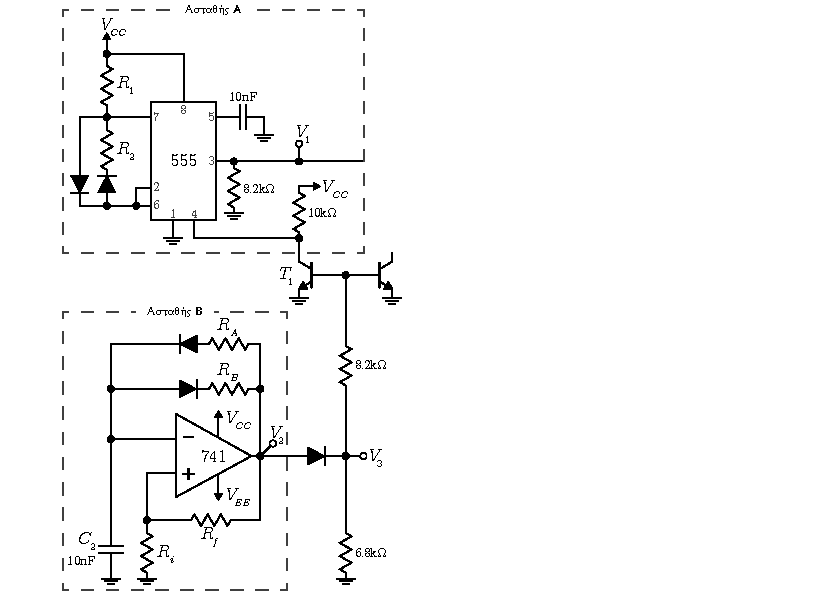
\includegraphics[width=14cm]{circuits/micro3_lab2.pdf}
		\caption{Γεννήτρια κλιμακωτής τάσης.}
		\label{circ:2_schematic}
	\end{circuitfig}
\end{center}

\section{Εργαστηριακή εφαρμογή}

	\subsection{Λήψη κυματομορφών $V_1$, $V_{C1}$ και $V_2$}
		Οι κυματομορφές $V_1$, $V_{C1}$ και $V_2$ του κυκλώματος \ref{circ:2_schematic}  δίδονται στο διάγραμμα \ref{plot:2.2_lab_voltages}.

		\begin{chart}[H]
			\begin{center}
				\pgfplotsset{grid style={dotted,lightgray}}
\begin{tikzpicture}
	\begin{axis}[
			scale only axis,
			height=4cm,
			width=5cm,
			grid=both,
			minor tick num=1,
			xtick={0,1,2,3,4,5,6,7,8,9,10,11,12,13,14},
			ytick={-1.8,0,5,10,13},
			xlabel={Time $\(\unit{\milli\second}\)$},
			ylabel={Voltage $\(\unit{\volt}\)$}]

		\addplot+[thick,mark=none,const plot,color=DodgerBlue3]
		coordinates	{(1.5+0,-1.8) (1.5+0,13) (1.5+0.450,13) (1.5+0.450,-1.8) (1.5+4.500,-1.8)
				(1.5+4.500,13) (1.5+4.950,13) (1.5+4.950,-1.8) (1.5+9.000,-1.8)};
		\legend{$v_1$}
	\end{axis}
\end{tikzpicture}\hspace*{1cm}
\begin{tikzpicture}
	\begin{axis}[
			scale only axis,
			height=4cm,
			width=5cm,
			grid=both,
			minor tick num=1,
			ymin=-2.4,
			ymax=3,
			samples=200,
			ytick={-2.32,-2,-1,0,1,2,2.88},
			xlabel={Time $\(\unit{\milli\second}\)$},
			ylabel={Voltage $\(\unit{\volt}\)$}]

		\addplot[thick,color=DeepPink3,domain=-0.2:0.2] {1.225+3.1*(1-exp(-x*3.81))};
		\addplot[thick,color=DeepPink3,domain=0.2:4.14] {-4.76+8.11*exp(-x*0.29)};
		\addplot[thick,color=DeepPink3,domain=-0.2+4.34:4.34+0.2] {1.225+3.1*(1-exp(-(x-4.34)*3.81))};
		\addplot[thick,color=DeepPink3,domain=0.2+4.34:4.14+4.34] {-4.76+8.11*exp(-(x-4.34)*0.29)};
		\legend{$v_{C_1}$}
	\end{axis}
\end{tikzpicture}\vspace*{0.5cm}
\begin{tikzpicture}
	\begin{axis}[
			scale only axis,
			height=4cm,
			width=8cm,
			grid=both,
			minor tick num=3,
			ymin=-5,
			ymax=25,
			ytick={-4,0,10,20,24},
			xlabel={Time $\(\unit{\milli\second}\)$},
			ylabel={Voltage $\(\unit{\volt}\)$}]

		\addplot+[thick,mark=none,const plot,color=SeaGreen4]
		coordinates	{(0,-4) (0,24) (3,24) (3,-4) (23.4,-4)
				(0+23.4,-4) (0+23.4,24) (3+23.4,24) (3+23.4,-4) (23.4*2,-4)};
		\legend{$v_2$}
	\end{axis}
\end{tikzpicture}
				\caption{Οι τάσεις $V_1$, $V_{C1}$ και $V_2$ όπως μετρήθηκαν χρήσει του παλμογράφου στο εργαστήριο.}
				\label{plot:2.2_lab_voltages}
			\end{center}
		\end{chart}

		Εφόσον η τροφοδοσία των τελεστικών ενισχυτών είναι $V_{CC}=15\unit{\volt}$ και $V_{EE}=-15\unit{\volt}$ είναι προφανές πως υπάρχει κάποιο offset στην τάση $V_2$ που παρατηρήθηκε στον παλμογράφο. καθώς η μέγιστη τιμή είναι $\max\(V_2\)=24\unit{\volt}>15\unit{\volt}$. Η σωστή κυματομορφή $V_2$ φαίνεται στο διάγραμμα \ref{plot:2.2b_lab_voltages}.\par
		\begin{chart}[H]
			\begin{center}
				\pgfplotsset{grid style={dotted,lightgray}}
\begin{tikzpicture}
	\begin{axis}[
			scale only axis,
			height=5cm,
			width=10cm,
			grid=both,
			minor tick num=3,
			ymin=-14,
			ymax=15.5,
			ytick={-12.8,-10,0,10,14.4},
			xlabel={Time $\(\unit{\milli\second}\)$},
			ylabel={Voltage $\(\unit{\volt}\)$}]

		\addplot+[thick,mark=none,const plot,color=SeaGreen4]
		coordinates	{(0,-12.8) (0,14.4) (3,14.4) (3,-12.8) (23.4,-12.8)
				(0+23.4,-12.8) (0+23.4,14.4) (3+23.4,14.4) (3+23.4,-12.8) (23.4*2,-12.8)};
		\legend{$V_2$}
	\end{axis}
\end{tikzpicture}
				\caption{Η σωστή τάση $V_2$.}
				\label{plot:2.2b_lab_voltages}
			\end{center}
		\end{chart}
